\documentclass{assets/utmreport}

\usepackage{booktabs,amssymb,float,graphicx,listings}

\hypersetup{hidelinks,hypertexnames=false,pdfauthor={Lucian-Adrian Gavril}}

\selectlanguage{english}

\utmlogo{assets/utm-logo.jpeg}

\institution{Technical University of Moldova}
\faculty{Faculty of Computers, Informatics, and Microelectronics}
\department{Department of Software Engineering}
\studyprogramme{Software Engineering Study Programme}
\documenttype{Laboratory report}
\reporttitle{Operating Systems Laboratories 5 \& 6}
\reportsubtitle{The File System with Your Own Hands and Inside the xv6 File System}
\student{Lucian-Adrian Gavril}{FAF-241}
\supervisor{Reițman Patricia}{univ. assist.}
\cityyear{Chișinău}{2026}

\setlength{\emergencystretch}{3em}

\begin{document}
\makeutmreporttitlepage
\tableofcontents
\clearpage

\begin{utmabstract}[Abstract]
This combined laboratory report investigates the principles, mechanisms, and internal structures of Unix filesystems across two distinct environments: the production Linux Virtual Filesystem (VFS) in Ubuntu 24.04 LTS (kernel 6.6.87.2 on x86\_64) and the educational MIT xv6 operating system running on an emulated RISC-V platform via QEMU 8.2.2.

Part I (Laboratory 5) examines the Linux filesystem from user space under an unprivileged user (\texttt{ubuntu}, UID 1000). It covers filesystem hierarchies, UsrMerge namespace unification, device inodes, inode-to-name decoupling, hard and symbolic link semantics, sparse file allocation, Discretionary Access Control (DAC) permission mechanics, and \texttt{/proc} introspection, including all four optional stretch problems (magic numbers, setuid auditing, open file descriptor unlinking, and loopback ext4 inode sizing).

Part II (Laboratory 6) dives into the xv6 filesystem internals. It analyzes on-disk directory tables, the structural layout of \texttt{struct dinode}, theoretical and physical capacity limits from \texttt{kernel/fs.h}, and the separation between directory unlinking in \texttt{sys\_unlink()} and block deallocation in \texttt{iput()} and \texttt{itrunc()}. Two user-space programs are implemented in C: \texttt{mystat.c} (inode and link inspection) and \texttt{find.c} (recursive directory search with the \texttt{-n} inode display stretch flag).
\utmkeywords{filesystems, linux, xv6, inodes, links, permissions, directory traversal}
\end{utmabstract}

\utmintroduction
This supplementary report documents the verified filesystem experiments across Linux VFS and xv6. The implementation details align with the included xv6 source\cite{xv6} and the individual Lab 5 and Lab 6 deliverables.

Filesystems are among the foundational abstractions of modern operating systems. They bridge persistent storage media and running processes by transforming raw block sectors into structured, human-navigable namespaces. Under Unix and POSIX semantics, filesystems extend beyond persistent disks: device drivers, interprocess communication pipes, and live kernel statistics all present uniform file descriptor interfaces.

This combined report documents the theoretical and practical investigation of both a full-scale production kernel (Linux) and an educational operating system (xv6):
\begin{utmenumerate}
\item \textbf{Laboratory 5 (Track A: Linux Warm-up)}: Direct shell inspection of filesystem types, inode table mechanics, hard and symbolic link lifecycles, space allocation in sparse files, Discretionary Access Control (DAC) permissions, process identification in \texttt{/proc}, and four advanced system experiments;
\item \textbf{Laboratory 6 (Track B: xv6 Filesystem Internals)}: Code-level tracing and live execution in the xv6 RISC-V kernel, developing \texttt{user/mystat.c} and \texttt{user/find.c}, evaluating on-disk block and inode layouts, analyzing link count decrement versus block deallocation timing, and exploring structural filesystem limits;
\end{utmenumerate}

\part{Laboratory 5: The File System with Your Own Hands (Linux)}

\chapter{Linux Filesystem Tree and File Types}

\section{System Root and Type Identification}
The leading character of an \texttt{ls -ld} listing identifies the inode type in the Linux VFS:
\begin{verbatim}
$ whoami
ubuntu

$ ls -ld /etc /etc/passwd /bin /dev/null /tmp
lrwxrwxrwx   1 root root    7 Apr 22  2024 /bin -> usr/bin
crw-rw-rw-   1 root root 1, 3 Oct 12 15:33 /dev/null
drwxr-xr-x 107 root root 4096 Oct 12 15:38 /etc
-rw-r--r--   1 root root 2430 Oct 12 15:38 /etc/passwd
drwxrwxrwt  10 root root 4096 Oct 12 15:38 /tmp
\end{verbatim}

\begin{figure}[H]
\centering
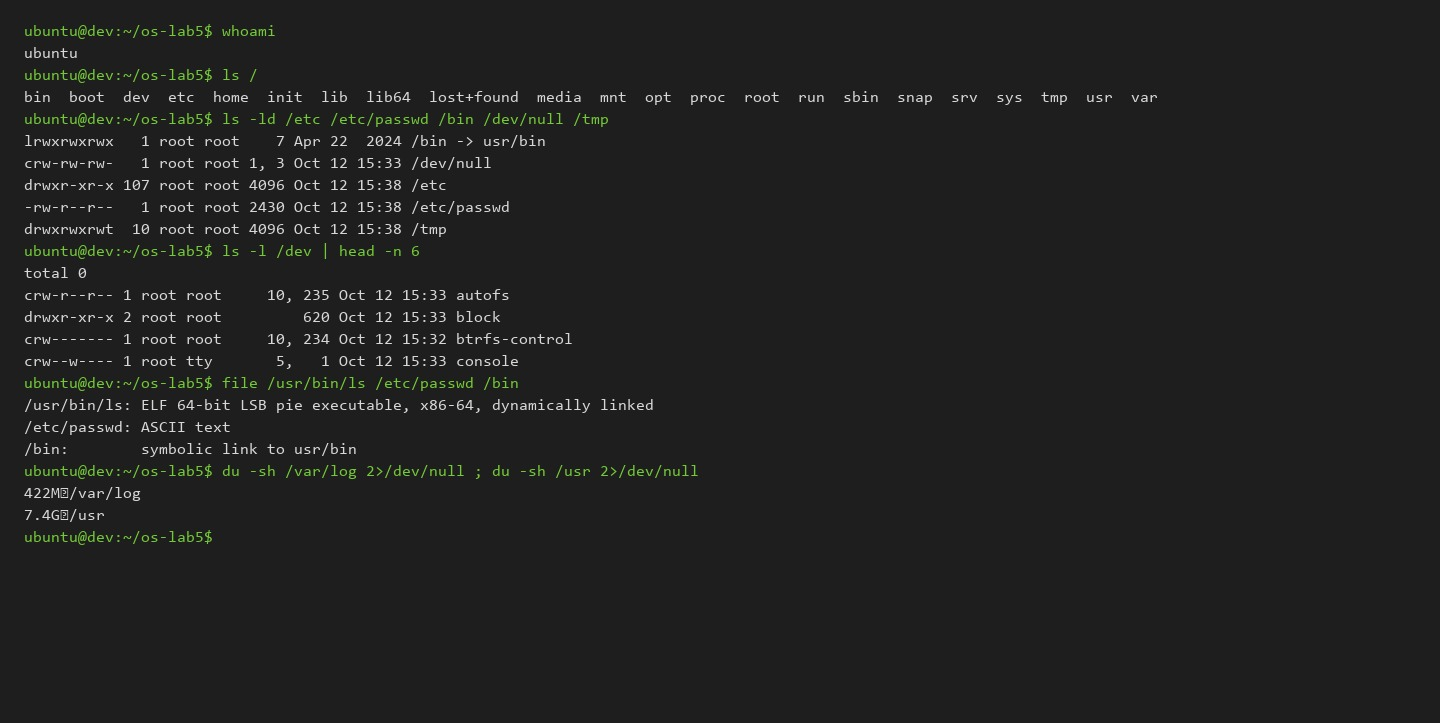
\includegraphics[width=0.92\textwidth]{assets/fig1_tree_and_types.jpg}
\caption{inspecting system root, device nodes, and file types.}
\label{fig:comb_l5_tree}
\end{figure}

\begin{table}[H]
\centering
\caption{Observed file types in Ubuntu 24.04 LTS}
\begin{tabular}{lcll}
\toprule
\textbf{Path} & \textbf{Type Char} & \textbf{Filesystem Type} & \textbf{Description} \\
\midrule
\texttt{/bin} & \texttt{l} & Symbolic Link & Points to \texttt{usr/bin} (UsrMerge) \\
\texttt{/dev/null} & \texttt{c} & Character Device & Byte-stream sink (major 1, minor 3) \\
\texttt{/etc} & \texttt{d} & Directory & System configuration tables \\
\texttt{/etc/passwd} & \texttt{-} & Regular File & User database in ASCII text \\
\texttt{/tmp} & \texttt{d} & Directory (Sticky) & World-writable temporary workspace \\
\bottomrule
\end{tabular}
\end{table}

\section{UsrMerge Architecture}
On modern Linux distributions, \texttt{/bin} is a symbolic link pointing to \texttt{usr/bin}. This design consolidates system software under \texttt{/usr}, simplifying package management, snapshotting, and read-only root mounting.

\section{Device Nodes in /dev}
Special device nodes do not consume disk blocks for file content. Instead, their inodes store major and minor numbers:
\begin{itemize}
\item \textbf{Character Device}: \texttt{/dev/null} (major 1, minor 3) and \texttt{/dev/console} (major 5, minor 1);
\item \textbf{Block Device}: \texttt{/dev/sda} (major 8, minor 0) and \texttt{/dev/sdd} (major 8, minor 48), supporting block-level operations through the page cache;
\end{itemize}

\section{Storage Comparison: /var/log vs /usr}
\begin{verbatim}
$ du -sh /var/log 2>/dev/null ; du -sh /usr 2>/dev/null
422M    /var/log
7.4G    /usr
\end{verbatim}
The \texttt{/usr} hierarchy occupies 7.4 GB, which is roughly 7.0 GB larger ($\approx 17.5 \times$) than \texttt{/var/log} (422 MB). This reflects \texttt{/usr}'s role in storing all system binaries, libraries, toolchains, and development headers.

\chapter{Inodes, Links, and Space Allocation}

\section{Inode Decoupling and Hard Link Creation}
Filenames are not stored inside inodes; they reside in directory tables as mapping entries:
\begin{verbatim}
$ echo hello > notes.txt
$ stat notes.txt
  File: notes.txt
  Size: 6           Blocks: 8          IO Block: 4096   regular file
Device: 8,48    Inode: 18829       Links: 1
\end{verbatim}

Creating a hard link creates an additional directory entry referencing the same inode:
\begin{verbatim}
$ ln notes.txt hard.txt
$ ls -li notes.txt hard.txt
18829 -rw-r--r-- 2 ubuntu ubuntu 6 Oct 12 15:39 hard.txt
18829 -rw-r--r-- 2 ubuntu ubuntu 6 Oct 12 15:39 notes.txt
$ rm notes.txt
$ cat hard.txt
hello
\end{verbatim}

\begin{figure}[H]
\centering
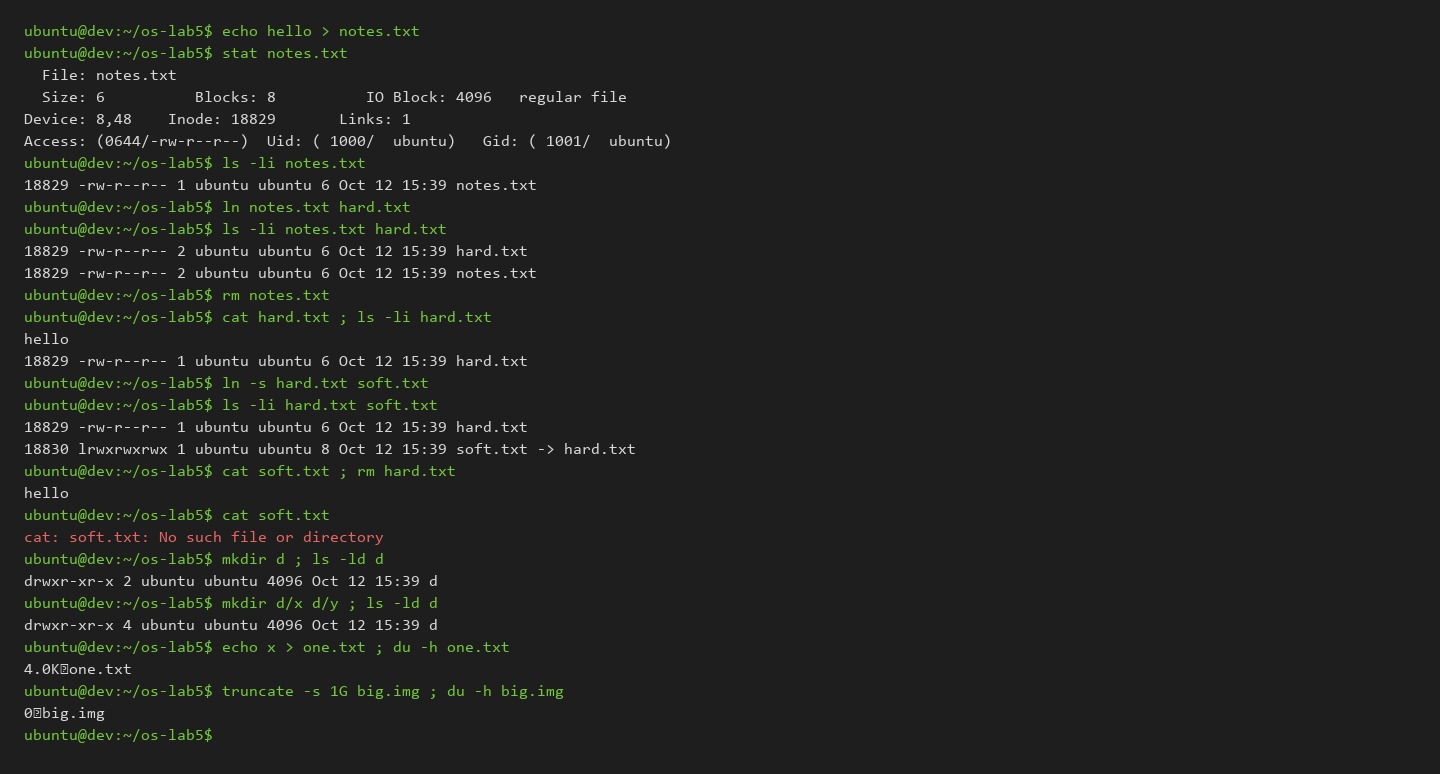
\includegraphics[width=0.92\textwidth]{assets/fig2_inodes_and_links.jpg}
\caption{inode inspection, hard links, dangling symlinks, and sparse files.}
\label{fig:comb_l5_inodes}
\end{figure}

The \texttt{rm} command unlinks the name \texttt{notes.txt} and decrements the inode link count from 2 to 1. Because \texttt{hard.txt} maintains a reference to inode 18829, the data blocks remain allocated and readable.

\section{Symbolic Link Semantics}
Symbolic links store the path of their target rather than referencing an inode number:
\begin{verbatim}
$ ln -s hard.txt soft.txt
$ ls -li hard.txt soft.txt
18829 -rw-r--r-- 1 ubuntu ubuntu 6 Oct 12 15:39 hard.txt
18830 lrwxrwxrwx 1 ubuntu ubuntu 8 Oct 12 15:39 soft.txt -> hard.txt
$ rm hard.txt
$ cat soft.txt
cat: soft.txt: No such file or directory
\end{verbatim}
Unlinking \texttt{hard.txt} leaves \texttt{soft.txt} dangling. The exact size of \texttt{soft.txt} is 8 bytes, matching the length of the string \texttt{"hard.txt"}.

\section{Directory Link Count Dynamics}
\begin{verbatim}
$ mkdir d ; ls -ld d
drwxr-xr-x 2 ubuntu ubuntu 4096 Oct 12 15:39 d
$ mkdir d/x d/y ; ls -ld d
drwxr-xr-x 4 ubuntu ubuntu 4096 Oct 12 15:39 d
\end{verbatim}
Under the classic ext-style directory link model, a directory starts with 2 links: its entry in the parent directory and the self-referencing `.` entry. Each subdirectory adds a `..` entry pointing back to the parent, incrementing the parent's link count to 4. This count is filesystem-dependent; it is not a universal Linux invariant.

\section{Sparse Files and Allocation Granularity}
\begin{verbatim}
$ echo x > one.txt ; du -h one.txt
4.0K    one.txt
$ truncate -s 1G big.img ; du -h big.img
0       big.img
\end{verbatim}
Ext4 allocates space in 4 KiB block increments, requiring 4.0 KiB even for a 2-byte file. In contrast, \texttt{truncate} creates a sparse file: it updates logical size metadata without writing data blocks, resulting in 0 physical blocks allocated.

\chapter{Permissions and System Introspection}

\section{Octal Modes and Owner Evaluation}
\begin{verbatim}
$ chmod 000 s.txt ; cat s.txt
cat: s.txt: Permission denied
\end{verbatim}
When the accessing user is the file owner, the kernel evaluates only the owner permission bits. Because they are \texttt{000}, access is denied. Ownership grants metadata authority (the right to invoke \texttt{chmod()}), not an automatic read bypass.

\begin{figure}[H]
\centering
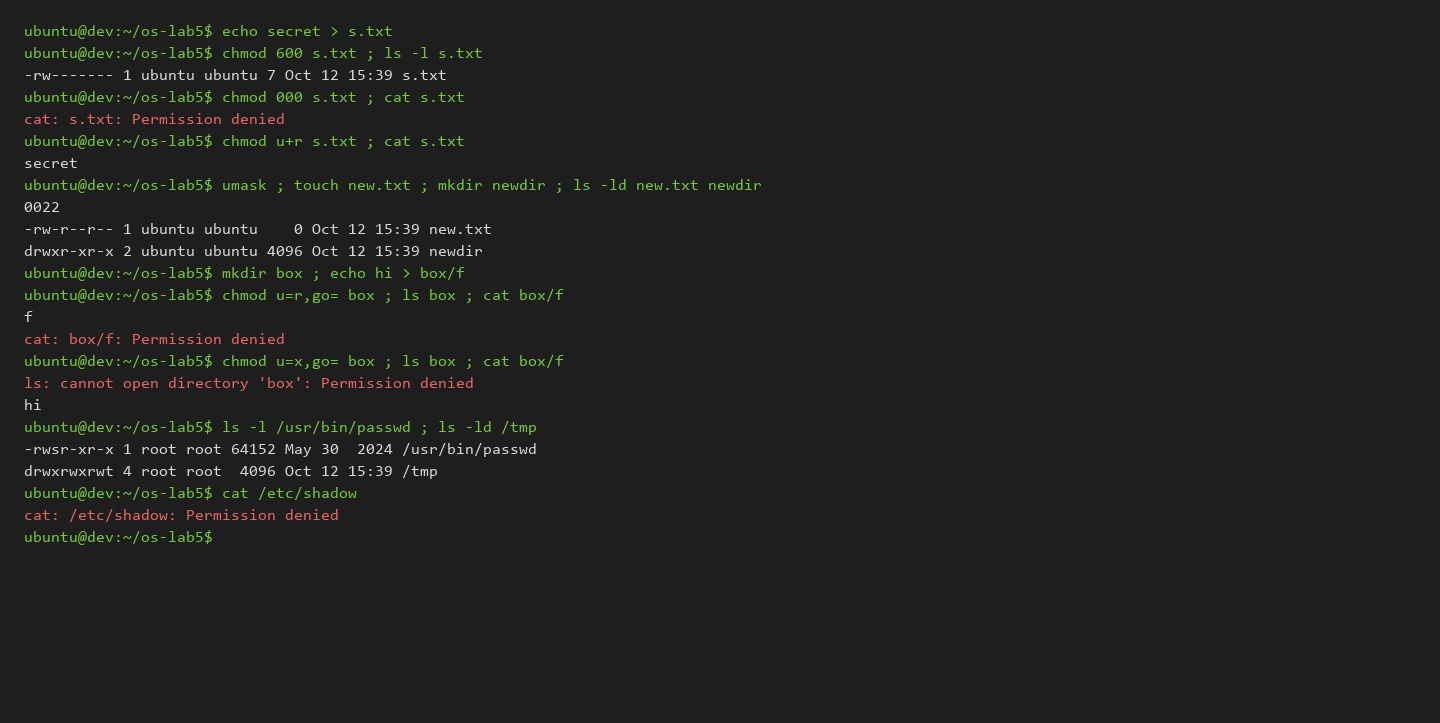
\includegraphics[width=0.92\textwidth]{assets/fig3_permissions.jpg}
\caption{permission evaluation, umask verification, and directory traversal.}
\label{fig:comb_l5_perm}
\end{figure}

\section{Umask Arithmetic}
The observed umask is \texttt{0022}. Files default to base mode \texttt{0666} ($0666 \ \& \ \sim 0022 = 0644$), while directories default to \texttt{0777} ($0777 \ \& \ \sim 0022 = 0755$).

\section{Directory Read versus Execute}
\begin{verbatim}
# Read-only directory
$ chmod u=r,go= box ; ls box ; cat box/f
f
cat: box/f: Permission denied

# Execute-only directory
$ chmod u=x,go= box ; ls box ; cat box/f
ls: cannot open directory 'box': Permission denied
hi
\end{verbatim}
Read permission (\texttt{r}) permits directory table enumeration, but accessing files inside requires execute permission (\texttt{x}) for path traversal.

\section{Setuid and Sticky Bit}
\texttt{/usr/bin/passwd} has setuid (\texttt{s}) to allow unprivileged users to update the root-owned \texttt{/etc/shadow} file. The sticky bit (\texttt{t}) on \texttt{/tmp} prevents users from deleting files owned by others.

\section{Disks, Topology, and /proc/self}
The system disk \texttt{/dev/sdd} (1 TB, ext4) is mounted at `/` with 1\% utilization (4.2 GB used). Introspection via \texttt{/proc} reveals 12 CPU cores and 19.38 GiB of RAM. Accessing \texttt{/proc/self/status} displays \texttt{Name: head} because \texttt{/proc/self} dynamically resolves to the PID of the accessing program.

\begin{figure}[H]
\centering
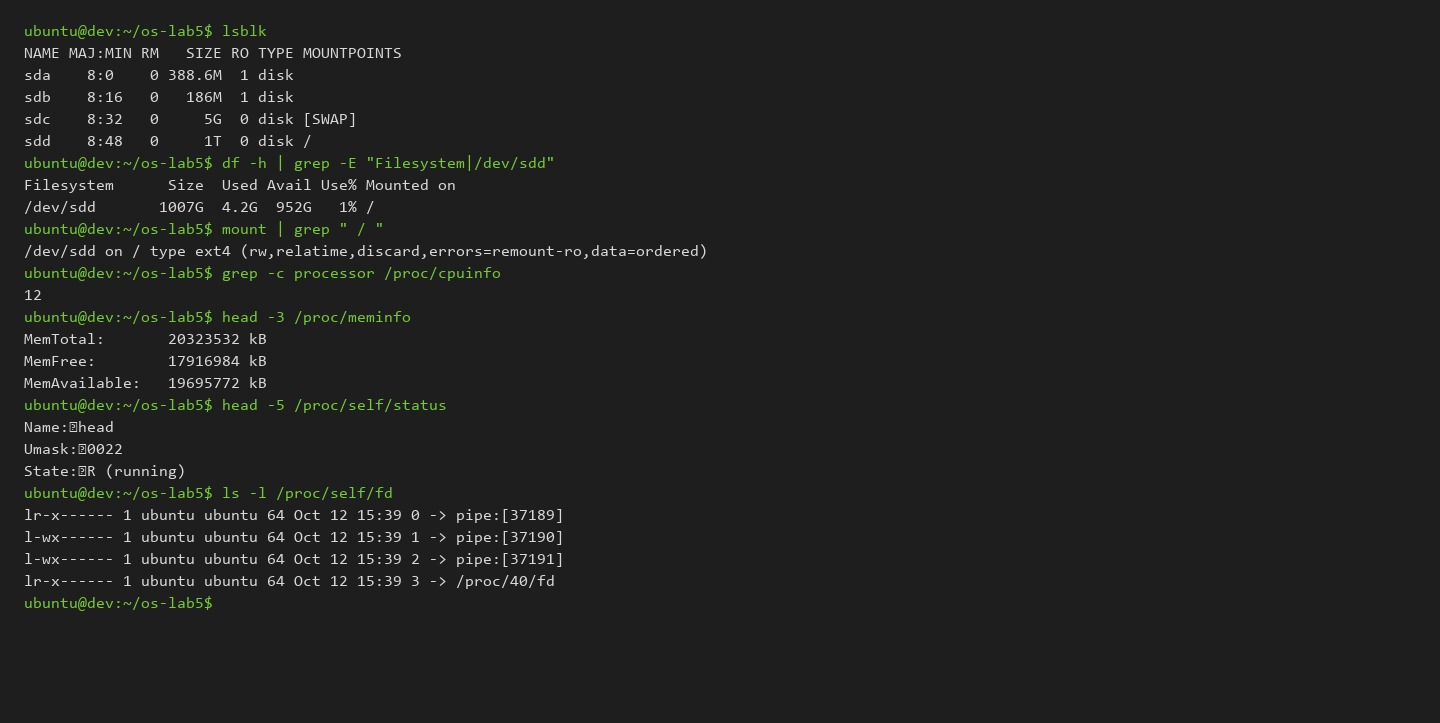
\includegraphics[width=0.92\textwidth]{assets/fig4_disks_and_proc.jpg}
\caption{disk topology, mount attributes, and procfs inspection.}
\label{fig:comb_l5_disks}
\end{figure}

\chapter{Laboratory 5 Stretch Problems}

\begin{figure}[H]
\centering
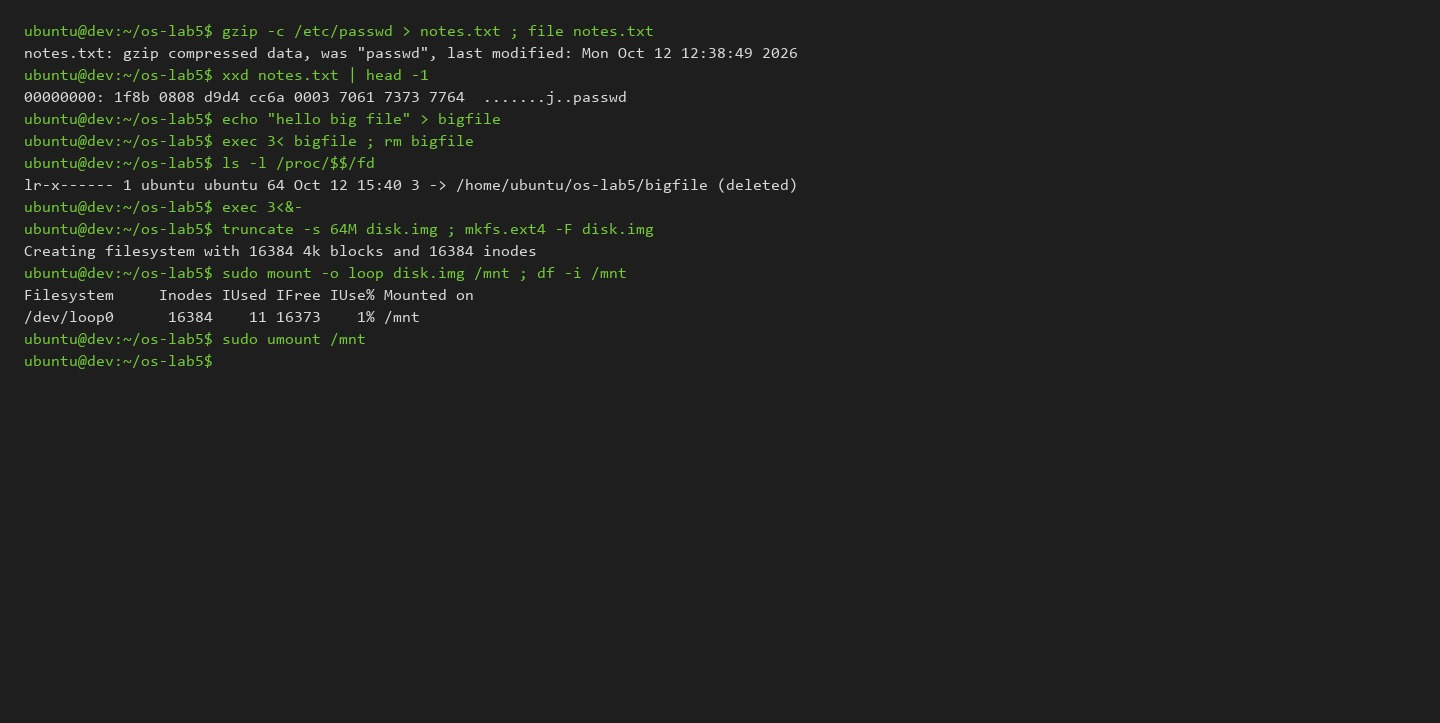
\includegraphics[width=0.92\textwidth]{assets/fig5_stretch.jpg}
\caption{magic bytes, unlinking open file descriptors, and ext4 loopback mount.}
\label{fig:comb_l5_stretch}
\end{figure}

\begin{itemize}
\item \textbf{(a) Magic Numbers}: Inspecting \texttt{notes.txt} via \texttt{xxd} reveals the leading bytes \texttt{0x1f 0x8b}, identifying the gzip compression format per RFC 1952;
\item \textbf{(b) Setuid Binaries}: Discovered setuid binaries include \texttt{passwd}, \texttt{su}, \texttt{sudo}, \texttt{mount}, \texttt{umount}, \texttt{polkit-agent-helper-1}, and \texttt{ssh-keysign};
\item \textbf{(c) Deleting Open Descriptors}: Unlinking an open file leaves \texttt{/proc/\$\$/fd/3 -> bigfile (deleted)}. Data blocks are freed only when descriptor 3 is closed via \texttt{exec 3<\&-};
\item \textbf{(d) Loopback Filesystem}: Creating a 64 MiB ext4 image formatted 16,384 inodes (one inode per 4 KiB block);
\end{itemize}

\part{Laboratory 6: Inside the xv6 File System}

\chapter{xv6 Directory Structure and Type Decoding}

\section{Filesystem Type Values}
xv6 defines three filesystem object types in \texttt{kernel/stat.h}:
\begin{verbatim}
#define T_DIR     1   // Directory
#define T_FILE    2   // Regular file
#define T_DEVICE  3   // Device
\end{verbatim}
Listing root in xv6 shows:
\begin{verbatim}
$ ls
.              1 1 1024
..             1 1 1024
README         2 2 2425
cat            2 3 35160
console        3 24 0
\end{verbatim}

\begin{figure}[H]
\centering
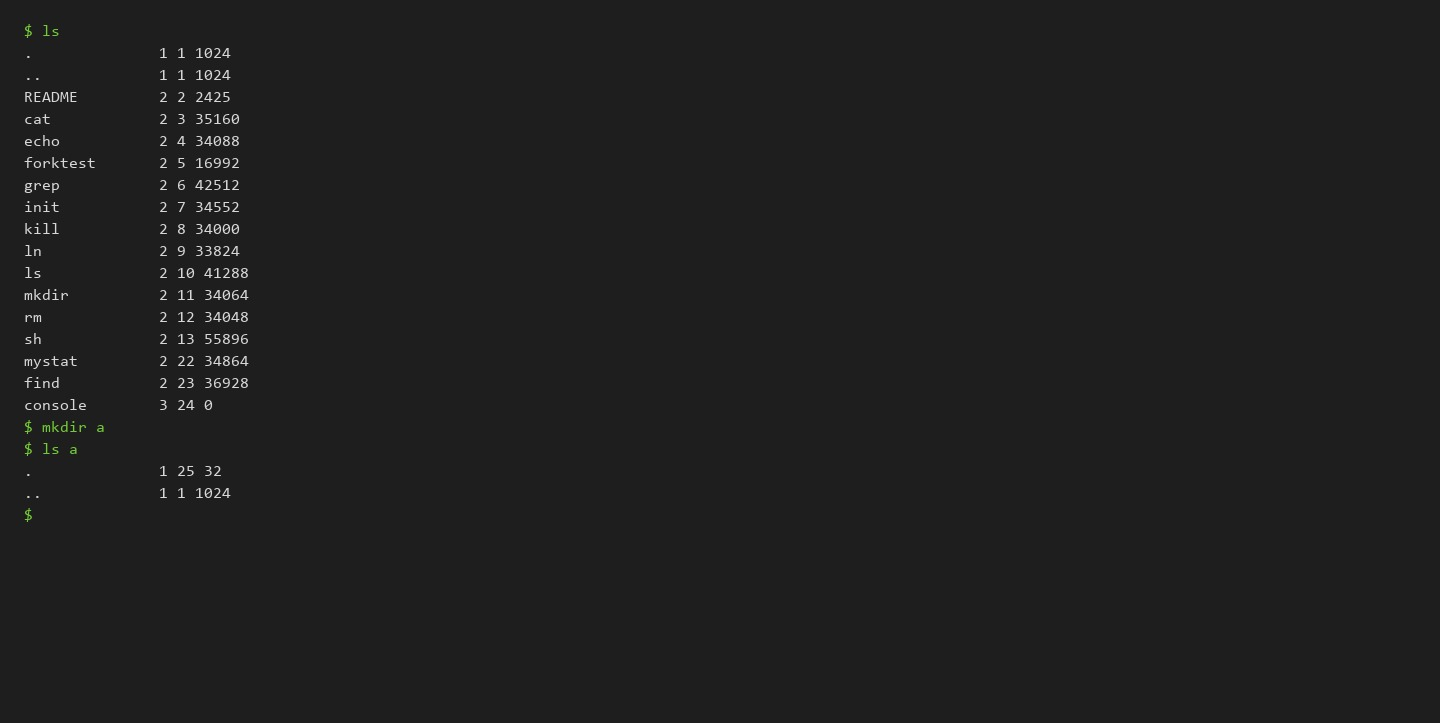
\includegraphics[width=0.92\textwidth]{assets/fig1_xv6_ls.jpg}
\caption{directory listing and type decoding in xv6.}
\label{fig:comb_l6_ls}
\end{figure}

\section{Root Directory and Entry Sizing}
The root directory resides at inode 1 (\texttt{ROOTINO = 1}). Both `.` and `..` point to inode 1 because the root has no parent. Each \texttt{struct dirent} is 16 bytes (2 bytes \texttt{inum} + 14 bytes \texttt{name}). An empty directory reports size 32 bytes, comprising exactly two 16-byte entries: `.` and `..`.

\chapter{The mystat Utility and Hard Link Mechanics}

\section{Implementation of user/mystat.c}
\begin{verbatim}
#include "kernel/types.h"
#include "kernel/stat.h"
#include "user/user.h"

char *typename(int t) {
  switch(t) {
  case T_DIR:    return "directory";
  case T_FILE:   return "file";
  case T_DEVICE: return "device";
  default:       return "?";
  }
}

int main(int argc, char *argv[]) {
  struct stat st;
  for(int i = 1; i < argc; i++){
    if(stat(argv[i], &st) < 0){
      fprintf(2, "mystat: cannot stat %s\n", argv[i]);
      continue;
    }
    printf("%s: %s, inode %d, links %d, size %ld bytes\n",
           argv[i], typename(st.type), st.ino, st.nlink, st.size);
  }
  exit(0);
}
\end{verbatim}

\section{Observing Hard Link Operations}
\begin{verbatim}
$ mystat README . console
README: file, inode 2, links 1, size 2425 bytes
.: directory, inode 1, links 2, size 1024 bytes
console: device, inode 24, links 1, size 0 bytes

$ ln README r2
$ mystat README r2
README: file, inode 2, links 2, size 2425 bytes
r2: file, inode 2, links 2, size 2425 bytes

$ rm README
$ mystat r2
r2: file, inode 2, links 1, size 2425 bytes

$ cat r2 | wc
48 334 2425
\end{verbatim}

\begin{figure}[H]
\centering
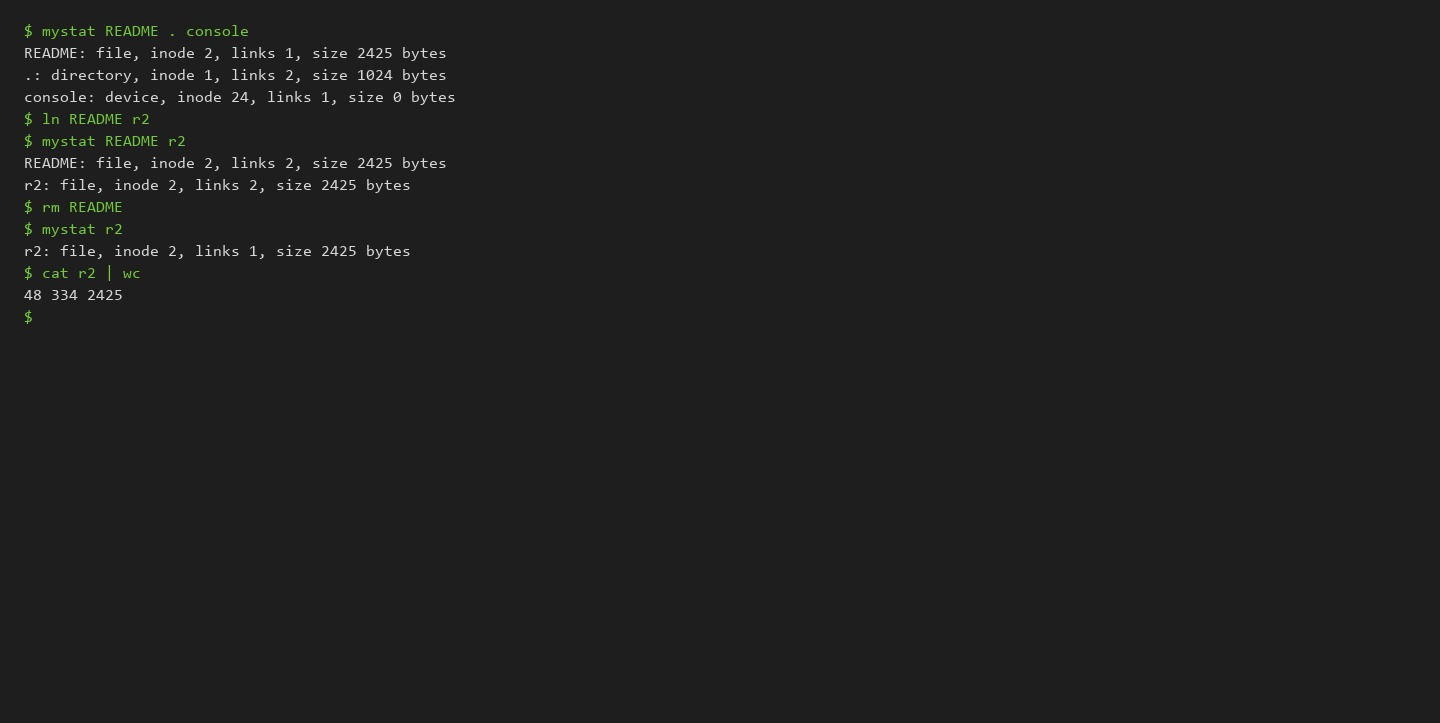
\includegraphics[width=0.92\textwidth]{assets/fig2_mystat_links.jpg}
\caption{mystat output, link counter increment, and unlinking.}
\label{fig:comb_l6_mystat}
\end{figure}

\section{Unlinking versus Deallocation}
In \texttt{kernel/sysfile.c}, \texttt{sys\_unlink()} decrements link count at line 230:
\begin{verbatim}
ip->nlink--;
iupdate(ip);
\end{verbatim}
Physical data blocks are deallocated only when \texttt{iput()} in \texttt{kernel/fs.c} determines that \texttt{ip->ref == 1} and \texttt{ip->nlink == 0}. It calls \texttt{itrunc(ip)}, which frees all direct and indirect blocks using \texttt{bfree()}.

\section{On-Disk Inode Structure}
In \texttt{kernel/fs.h}, \texttt{struct dinode} contains:
\begin{verbatim}
struct dinode {
  short type;              // File type
  short major;             // Major device number (T_DEVICE only)
  short minor;             // Minor device number (T_DEVICE only)
  short nlink;             // Hard link counter
  uint size;               // File size in bytes
  uint addrs[NDIRECT+1];   // Block addresses (12 direct + 1 indirect)
};
\end{verbatim}
xv6 inodes omit permissions, UIDs, timestamps, and symbolic links.

\chapter{Limits and Disk Architecture}

\section{Filename Truncation}
The directory format stores at most \texttt{DIRSIZ = 14} name bytes. The example name \texttt{averyveryvery\allowbreak{}longname} is therefore stored as \texttt{averyveryveryl}, its first 14 characters.

\section{Maximum File Capacity}
\begin{itemize}
\item Block size: $\text{BSIZE} = 1024\text{ bytes}$;
\item Direct blocks: $\text{NDIRECT} = 12$ blocks ($12\text{ KiB}$);
\item Indirect blocks: $\text{NINDIRECT} = 1024 / 4 = 256$ blocks ($256\text{ KiB}$);
\item Total blocks: $12 + 256 = 268$ blocks ($274,432\text{ bytes} \approx 268\text{ KiB}$);
\end{itemize}

\begin{figure}[H]
\centering
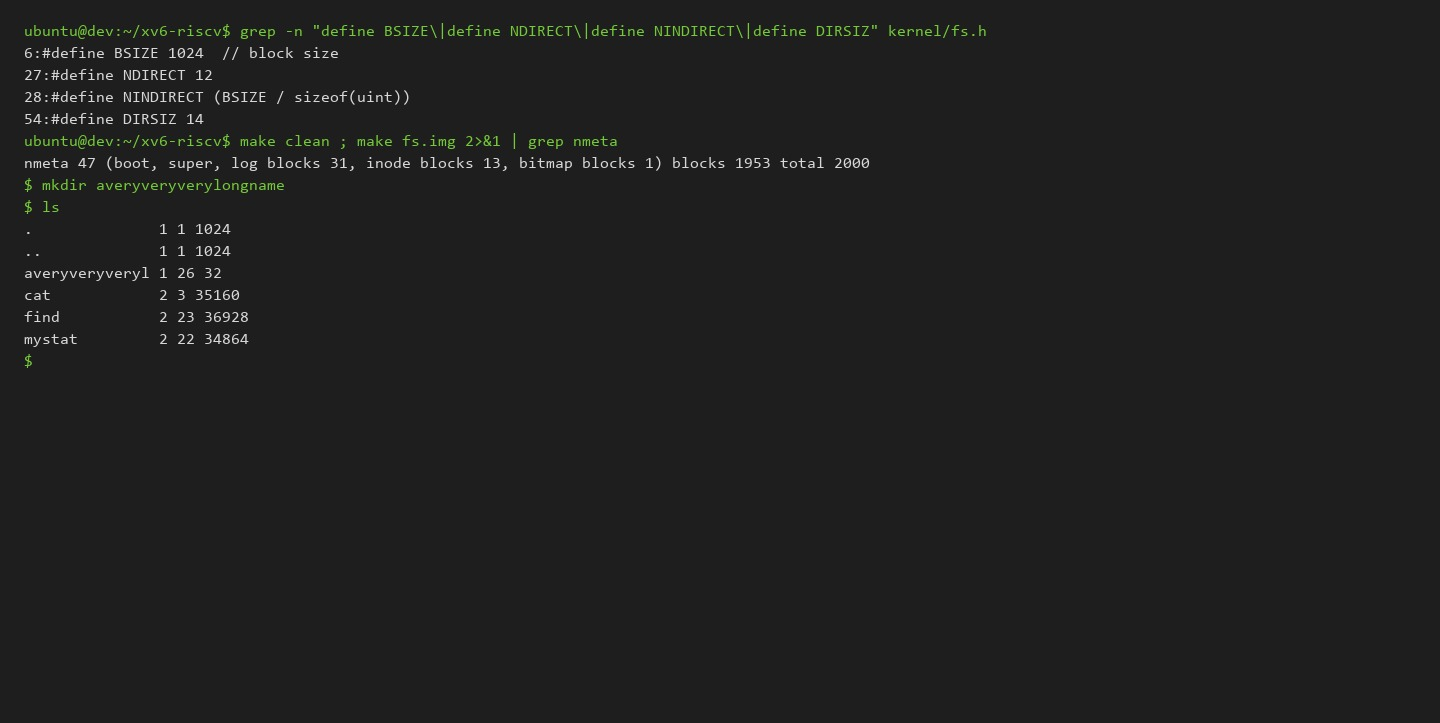
\includegraphics[width=0.92\textwidth]{assets/fig3_limits_truncation.jpg}
\caption{measuring constants, disk layout, and 14-byte truncation.}
\label{fig:comb_l6_limits}
\end{figure}

\section{Disk Layout}
\texttt{mkfs} reports:
\begin{verbatim}
nmeta 47 (boot, super, log blocks 31,
  inode blocks 13, bitmap blocks 1)
blocks 1953 total 2000
\end{verbatim}
Total disk size is 2000 blocks. 47 blocks are reserved for metadata (one boot block, one superblock, 31 log blocks, 13 inode blocks and one bitmap block). The remaining 1953 blocks form the data region; this does not mean they all contain allocated file data.

\chapter{Recursive Search: user/find.c and Inode Verification}

\section{Implementation of user/find.c}
The \texttt{find} program recurses through directory trees while strictly closing file descriptors to prevent descriptor exhaustion:
\begin{verbatim}
#include "kernel/types.h"
#include "kernel/stat.h"
#include "user/user.h"
#include "kernel/fs.h"
#include "kernel/fcntl.h"

static int show_ino = 0;

void find(char *path, char *target) {
  char buf[512], *p;
  int fd;
  struct dirent de;
  struct stat st;

  if((fd = open(path, O_RDONLY)) < 0) return;
  if(fstat(fd, &st) < 0 || st.type != T_DIR) { close(fd); return; }

  strcpy(buf, path);
  p = buf + strlen(buf);
  *p++ = '/';

  while(read(fd, &de, sizeof(de)) == sizeof(de)){
    char name[DIRSIZ + 1];
    if(de.inum == 0) continue;
    memmove(name, de.name, DIRSIZ);
    name[DIRSIZ] = 0;
    if(strcmp(name, ".") == 0 || strcmp(name, "..") == 0) continue;

    strcpy(p, name);
    if(stat(buf, &st) < 0) continue;
    if(strcmp(name, target) == 0){
      if(show_ino) printf("%s %d\n", buf, st.ino);
      else printf("%s\n", buf);
    }
    if(st.type == T_DIR) find(buf, target);
  }
  close(fd);
}
\end{verbatim}

\section{Testing and Inode Stretch Resolution}
\begin{verbatim}
$ mkdir a
$ mkdir a/b
$ echo x > a/b/r2
$ echo y > a/r2
$ ln cat r2

$ find . r2
./r2
./a/b/r2
./a/r2

$ find a b
a/b

$ find . r2 -n
./r2 3
./a/b/r2 26
./a/r2 27

$ mystat cat
cat: file, inode 3, links 2, size 35160 bytes
\end{verbatim}

\begin{figure}[H]
\centering
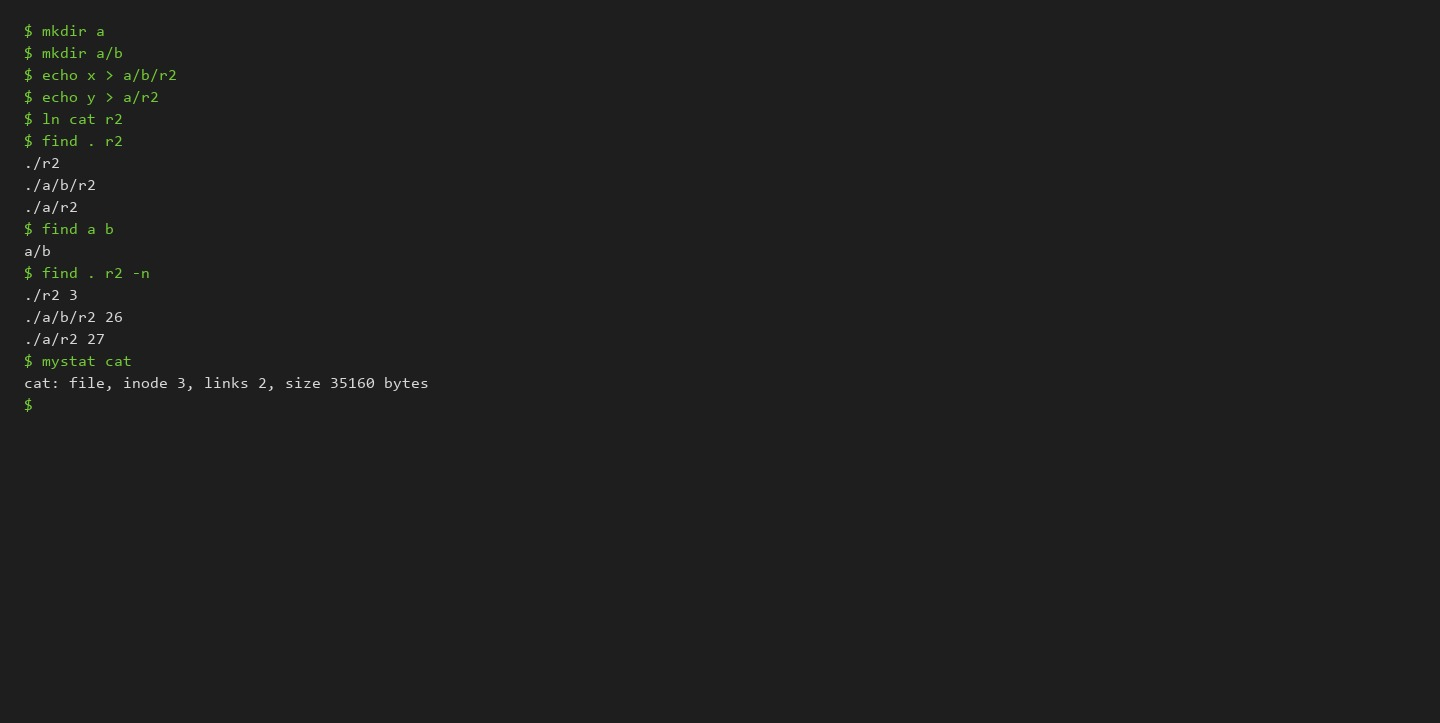
\includegraphics[width=0.92\textwidth]{assets/fig4_find_and_stretch.jpg}
\caption{find execution and -n stretch proving inode identity.}
\label{fig:comb_l6_find}
\end{figure}

The saved \texttt{-n} example illustrates that \texttt{./r2} and \texttt{cat} share inode 3 and link count 2, confirming they are identical files on disk. The files \texttt{a/b/r2} (inode 26) and \texttt{a/r2} (inode 27) are distinct newly created files.

\utmconclusions
This combined investigation demonstrates how filesystem abstractions are realized in production and educational operating systems. In both Linux and xv6, directory tables decouple human-readable names from inode metadata. Hard links manipulate link counters without duplicating disk blocks, and physical block deallocation occurs only when all links and open process descriptors are released.

\begin{thebibliography}{9}
\bibitem{xv6} MIT PDOS. \textit{xv6-riscv source code}. Included course snapshot in \texttt{lab2/}; \texttt{kernel/fs.c}, \texttt{kernel/fs.h}, and \texttt{kernel/sysfile.c}. Source inspected 23 October 2026. \url{https://github.com/mit-pdos/xv6-riscv}.
\end{thebibliography}
\end{document}
